
\documentclass[PICOReport.tex]{subfiles}

\begin{document}

%Enumerate the various signals in polarization. Use the frequency band + signals figure. The challenge is to dig out the faintest of all signals, the one due to $r$. This sets the tone for the entire 'signal decomposition' or 'component separation'.  Removing the galactic signal to unmask $r \lesssim 0.001$ is a challenge for all future experiments searching for $r$ at that level, and is a strong advantage of a space platform. The physics of galactic signals suggests complexities in their combined emission properties; the level of this complexity is not known. } 

\subsubsection{The Signal Separation Challenge}
\label{sec:separation_challenge}

In the PICO frequency range there are Galactic and extragalactic sources of emission. Galactic emissions are due to free-free, synchrotron, and dust, which arise respectively from photon emission in free electron-proton scattering, free electrons spiraling around Galactic magnetic field lines, and from $\sim$20~K elongated interstellar dust grains partially aligned with the local magnetic field. Free-free emission is expected to have negligible polarization. The emission from synchrotron and dust are linearly polarized, and has both $E$ and $B$ components (Fig.~\ref{fig:pico-channels-and-fg}).  Extragalactic sources of emission include the CMB, which has both $E$ and $B$ modes, and point sources %various types 
whose polarization level and type are not well constrained. The task of `separating the signal to its components' (sometimes shortened to `component separation') is to decompose the detected signal to its constituent sources. The required precision of signal separation is determined by the requirement to detect or set an upper limit on the inflationary $B$-mode, which is the faintest among PICO's targeted signals. In that context, the terms `foreground separation' and `foreground cleaning' are used as equivalents to `signal separation'. 

Galactic emission dominates the sky's polarized intensity on large angular scales ($\ell \lesssim 10$), it dominates the cosmological $B$-modes signals for $\ell \lesssim 150$ for all allowed levels of $r$, and it is expected to be significant even at $\ell \simeq 1000$, posing challenge for reconstructing the $B$-mode signal from lensing. This is illustrated in Figs.~\ref{fig:clbb} and~\ref{fig:pico-channels-and-fg}, which show Galactic emission power spectra calculated for the cleanest -- that is, the least Galactic-emission-contaminated -- 60\% of the sky. But even in small patches of the sky, far from the Galactic plane and with the least foreground contamination, Galactic emission levels are substantial relative to an inflationary signal of $r \sim 0.01$ and overwhelm it for $r \lesssim 0.001$~\cite{planckEB}. Separating the cosmological and Galactic emission signals is {\it the} primary challenge facing any next-decade experiment attempting to reach these levels of constraints on $r$, along with control of systematic uncertainties.

\begin{figure}[ht]
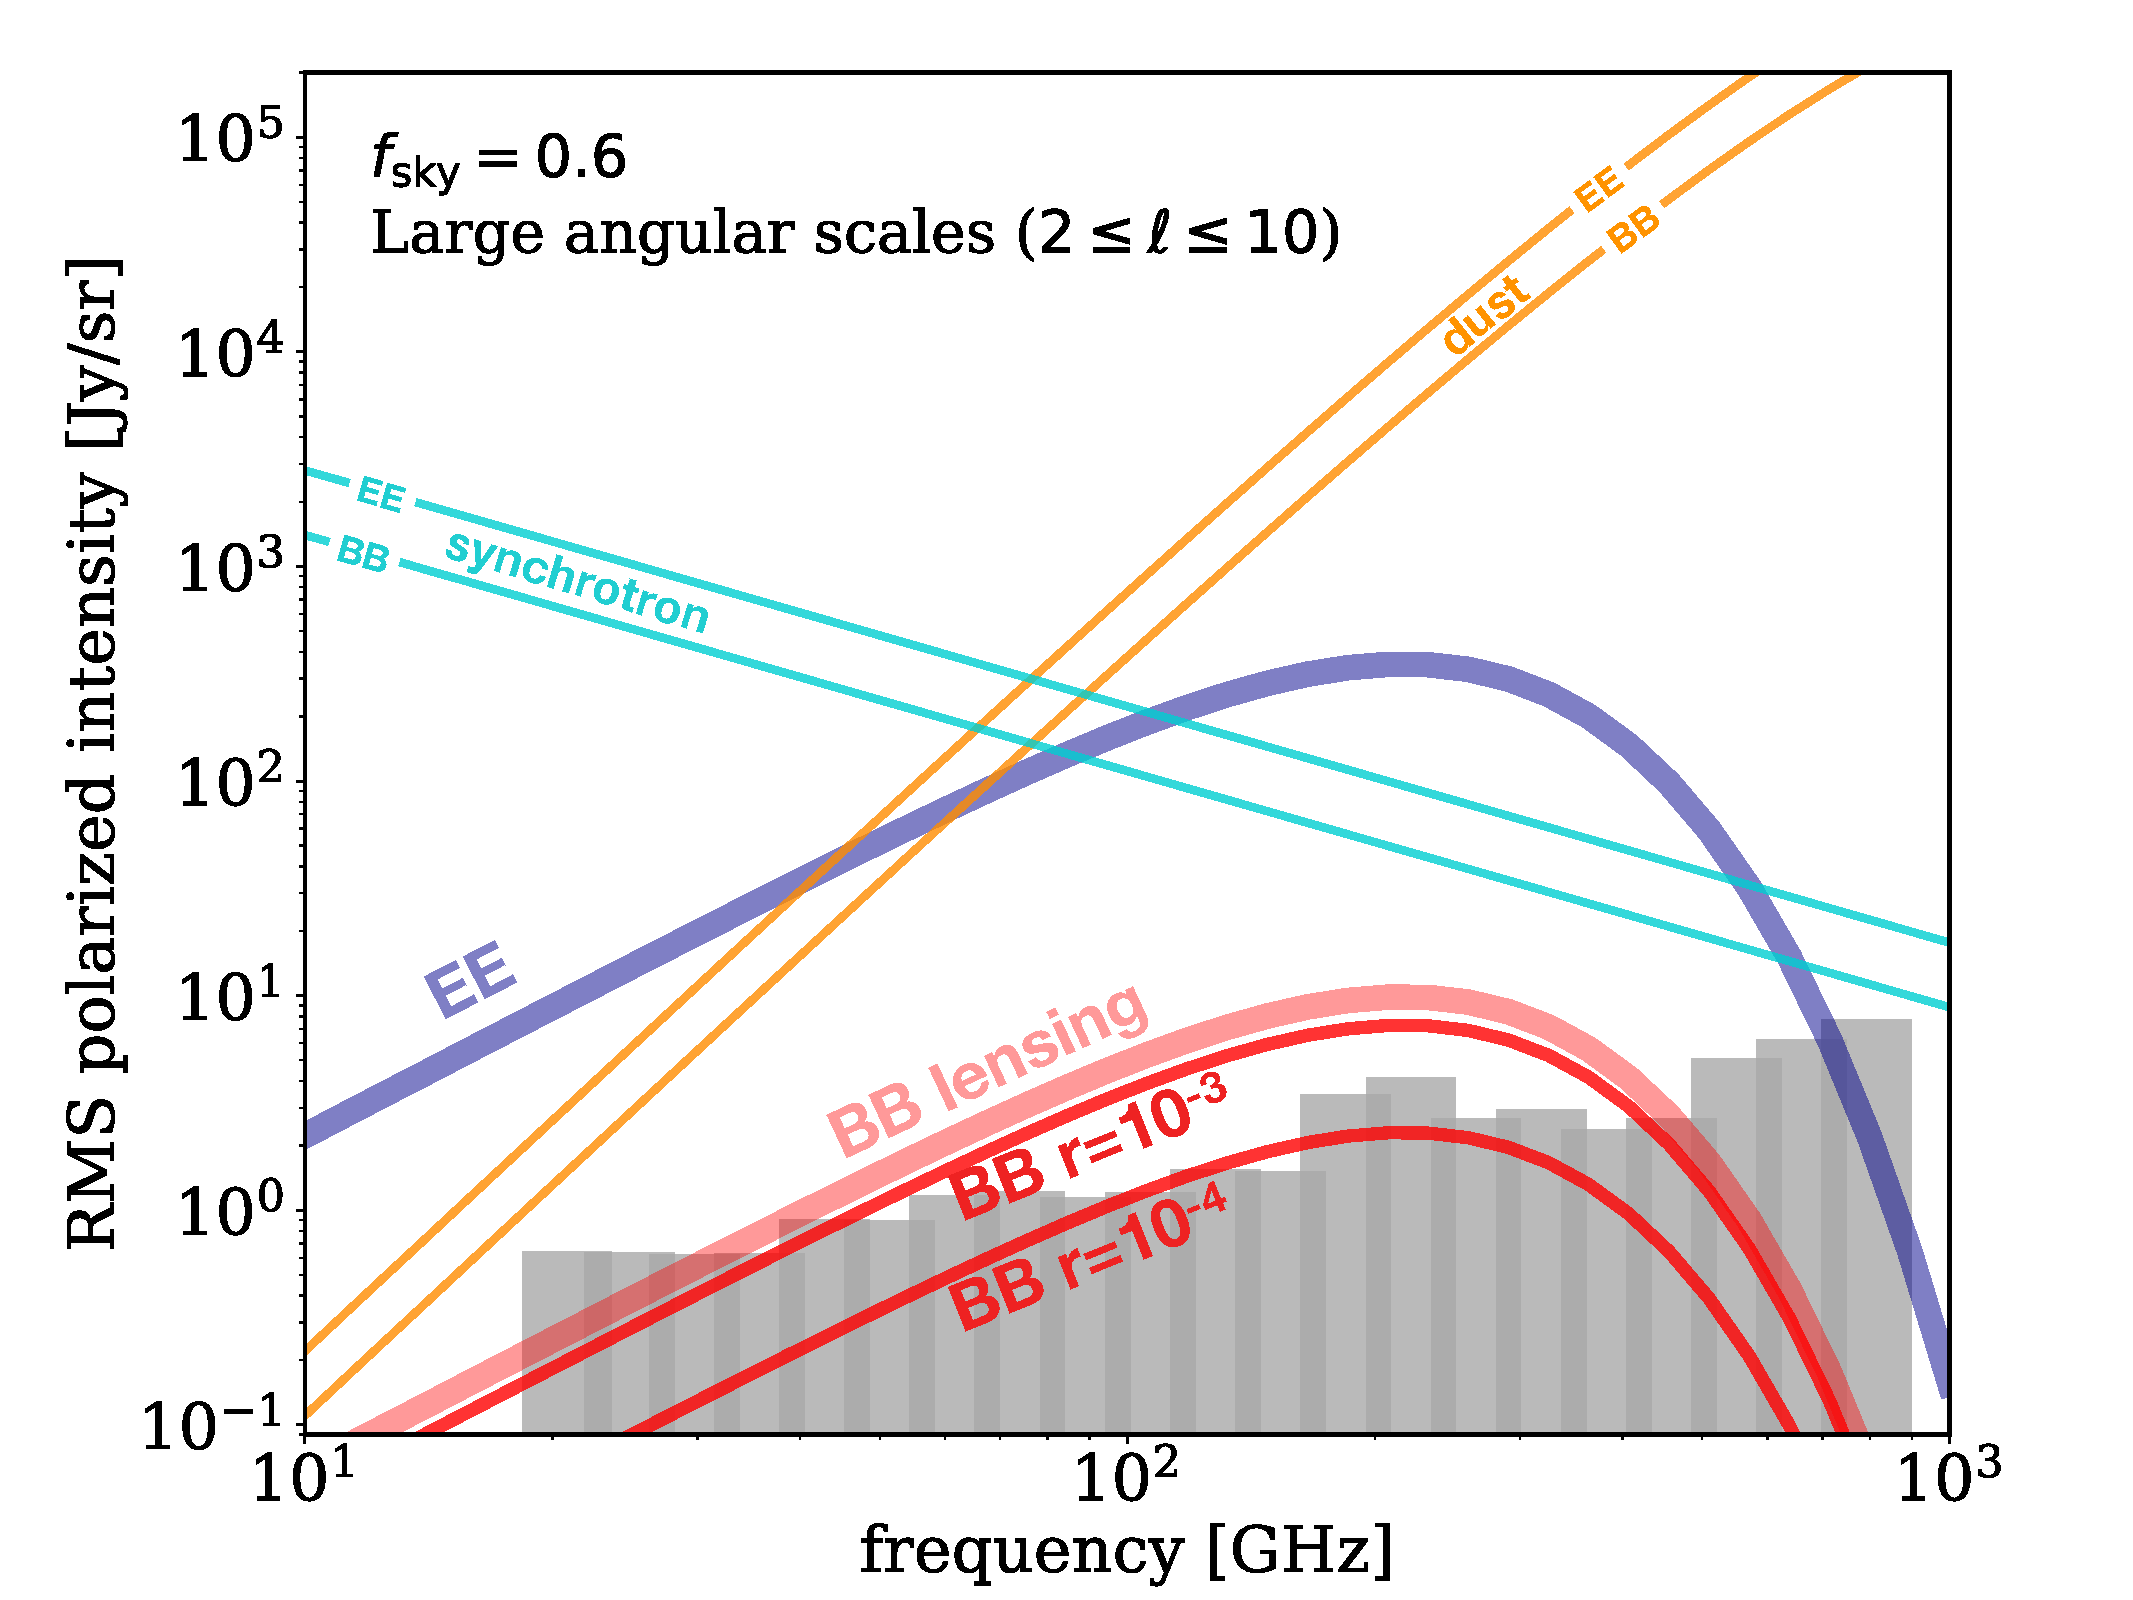
\includegraphics[width=0.49\textwidth]{images/sensitivity_vs_frequency_Jan3_2019_large_scale_v2.pdf}
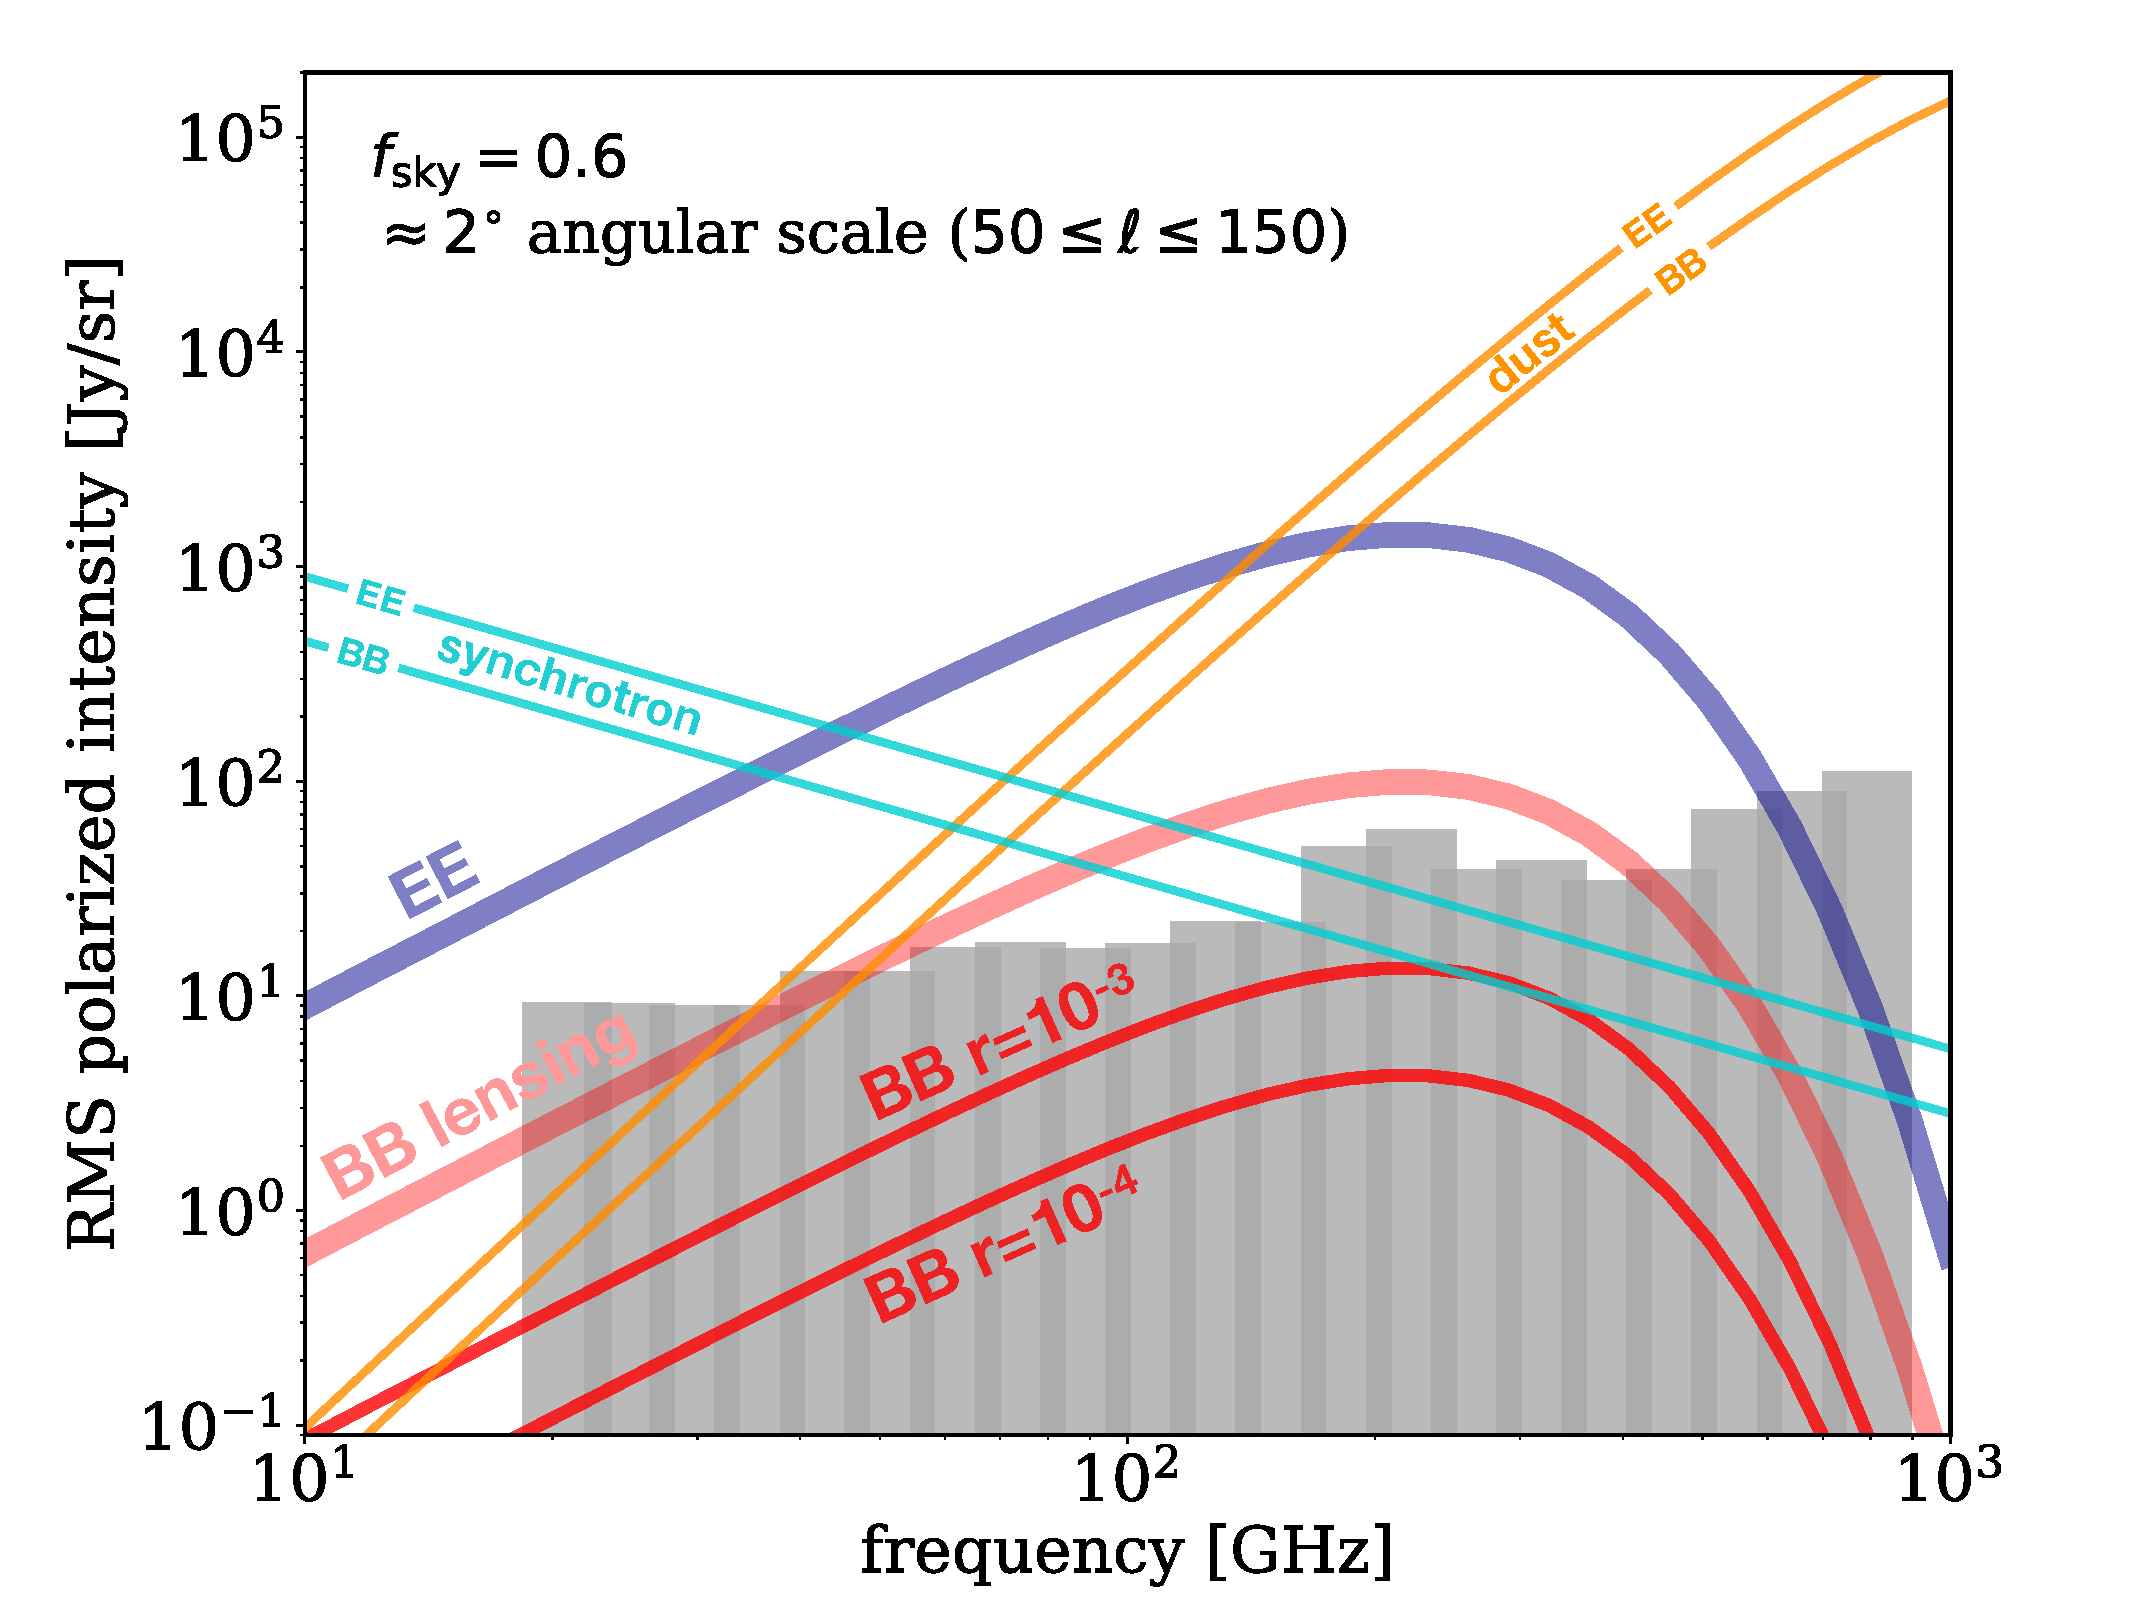
\includegraphics[width=0.49\textwidth]{images/sensitivity_vs_frequency_Jan3_2019_2deg_scale_v2.pdf}
\vspace{-0.1in}
\caption{\captiontext
Polarization $BB$ spectra of Galactic synchrotron and dust, compared to CMB polarization $EE$ and $BB$ spectra of different origins for two values of $r$ and for two ranges of angular scales: large-scale, $\ell \leq 10$, corresponding to the reionization peak (left panel); and intermediate scales $50 \leq \ell \leq 150$, corresponding to the recombination peak (right panel). 
Data from \planck\ indicate that for Galactic emission the level of the $E$-mode is approximately twice that of $B$~\cite{planckEB}.
The PICO baseline noise (grey bands) is low compared to the Galactic emission components, and thus they will be measured with high \ac{SNR} in many frequency bands.
\label{fig:pico-channels-and-fg} }
\vspace{-0.05in}
\end{figure}

Foreground separation is challenging because the spatial power spectra and frequency spectra of the foregrounds are not known to sufficient accuracy anywhere across the sky.
%Galactic emissions are neither precisely characterized spatially, nor do they have , or were known to have simple, fittable spectral emission laws they could be separated. But neither is true. 
To a first approximation, the spectrum of synchrotron emission is a power law $I_{\rm sync} \propto \nu^{\alpha},$ with $\alpha \simeq -1$.  The spectrum of dust emission is $I_{\rm dust} \propto \nu^{\beta} B_\nu(T_{\rm dust}),$ where $\beta \simeq 1.6$, $T_{\rm dust} \simeq 20$\,K, and $B_\nu(T)$ is the Planck function; this is referred to as `modified blackbody emission'. If those models exactly reflected the properties of emitting sources, then in principle an experiment that had six frequency bands could determine the three emission parameters, as well as the three amplitudes for the dust, synchrotron, and CMB components. However, recent observations have shown that neither emission law is universal, that spectral parameters are not necessarily the same for intensity and polarization and that they vary across the sky \cite{SPASS_2018_variation,fuskeland2014_wmap_variation,planck_2013_xi}, and thus that the analytic forms and parameter values given above are only approximately valid for averages across the sky~\citep{chluba2017foregrounds}. Also, while both emission laws are well-motivated phenomenological descriptions, the fundamental physics of emissions from grains of different materials, sizes, and temperatures, and of electrons spiraling around magnetic fields, implies that these laws are expected to be neither exact, nor universal. 

At the low levels of $r$ targeted by PICO and by other next-decade experiments, even small inaccuracies in foreground modeling and characterization lead to biases and false detections. Several publications have demonstrated that fitting complicated dust temperature profiles using a simple one- or two-temperature model will bias the fitted CMB signal at levels $\delta r \lesssim 10^{-3}$, which is significant compared to PICO's goal~\citep{fantaye2011,armitage-caplan2012,kogut_fixsen2016,remazeilles/etal:2016,stompor2016}. 

%We can no longer impose specific models upon the data; rather, the data collected should provide information to constrain Galactic emissions with sufficient accuracy. 

% and other next decade will dramatically improve sensitivity to inflationary B-modes. The improved sensitivity requires concurrent improvements in foreground separation.  Simple foreground models, suitable for the current generation of CMB measurements, will fail at the higher PICO sensitivity.  For example, the \planck~modified blackbody model assumes that interstellar dust emits at a single temperature, which is clearly an approximation to the more complicated emission along lines of sight spanning hundreds of parsecs. Several publications have demonstrated that fitting complicated temperature profiles using a simple one- or two-temperature model will bias the fitted CMB signal at levels $\delta r \lesssim 10^{-3}$, large compared to the PICO goal~\citep{fantaye2011,armitage-caplan2012,kogut_fixsen2016,remazeilles/etal:2016,stompor2016}.

Further complicating the foreground-separation challenge is the fact that additional polarized foregrounds may exist.  
%`Anomalous microwave emission' (AME) has been observed at mm wavelengths, spatially correlated with thermal dust emission, but with intensity peaking at frequencies near 30 GHz.
Anomalous microwave emission (AME), dust-correlated emission peaking in intensity near 30~GHz, is an important low-frequency foreground in total intensity. 
It has been tentatively attributed to small, rapidly-spinning dust grains~\citep{dickinson2018}. Current $1\sigma$ upper limits on AME polarization are at the level of 1\%~\citep{dickinson2018}. If it is 1\% 
%Very few measurements of AME polarization exist, and there are only loose constraints on its fractional polarization; it is less than 3\% (2$\sigma$) at 18~GHz in one 0.5\% region of the sky~\citep{genova_santos:2015}.  If AME is 1\% 
polarized, left uncorrected it would give rise to a bias of $\delta r \simeq 5\times10^{-4}$~\citep{remazeilles2016}.  Astrophysical emission from CO lines at mm wavelengths is expected to be 0.1--1\,\% polarized~\citep{greeves1999, puglisi2017}.  Extragalactic radio sources show a median polarization of 2\%~\citep{Bonavera2018, puglisi2018_polsource, trombetti2018_fracpol}, and there is significant uncertainty about the polarization of dusty galaxies emitting in the PICO wavebands. Initial quantitative estimates show that ignoring radio sources and dusty galaxies may each lead to a bias $\delta r > 3\times10^{-3}$~\citep{toffolatti2012,Bonavera2018,remazeilles2018}  %at $\ell=80$ 
at low and high frequencies, respectively, and ignoring the CO\,$J=1\rightarrow0$ line could lead to a bias $\delta r > 2\times10^{-3}$~\citep{puglisi2017} at 115~GHz. % and the same $\ell$ range. 
These levels are appreciable compared to the goals of PICO and other next-decade experiments. 

%%%%%%%%%%%%%%%%%%%%%%%%%%%%%%%%%%%
\subsubsection{Foreground Separation Assessment and Methodology}
\label{sec:foreground_separation_methodology}
%%%%%%%%%%%%%%%%%%%%%%%%%%%%%%%%%%%


%Faced with these uncertainties, but also with the opportunity provided by a platform that can host a broad range of frequencies -- ground-based experiments are limited to several atmospheric windows and to frequencies of less than 300~GHz -- PICO is designed with 21 frequency bands between 21 and 800 GHz; see Fig.~\ref{fig:pico-channels-and-fg} and Table 3.2. This is the broadest frequency lever arm proposed by any imaging instrument to characterize and enable separation of Galactic emissions. 

%The level of fidelity required in the characterization of foreground emissions compels new approaches to the way we assess and forecast the performance of a future experiment. We can no longer impose specific models upon the data; rather, the data collected should provide information to constrain Galactic emissions with sufficient accuracy.  

%Two broad approaches are used for foreground separation and for assessment of its precision.  In the parametric approach the foregrounds are assumed to follow emission laws described by a number of free parameters. Parametric models use the frequency dependence of the data in each line of sight to determine the values of the parameters~\citep{eriksen/etal:2008}.  Since the CMB spectrum is well determined, measurements with a sufficient number of frequency bands and appropriately broad frequency coverage can distinguish foreground emission from the CMB using their different spectral dependences. Non-parametric techniques, in contrast, rely on the fact that CMB emission is uncorrelated with the foregrounds and thus correlations within a given spatial/frequency data-cube can be used to separate the two distinct sources of emission~\citep{delabrouille2003,Cardoso2008,Delabrouille2009,nilc,gnilc}.  Simulated data are used to assess the efficacy of both techniques as the complexity of the assumed foreground emission is increased. For the parametric models, we can also employ analytic methods to estimate the uncertainty on emission parameters as a function of instrument noise, but specific assumptions must be made about the underlying nature of the emission laws~\citep{errard_and_finney}. 

To investigate the efficacy of PICO in addressing the foreground-separation challenge, we used both an analytic forecast and map-domain simulations. \\ 
%
\noindent$\bullet$ {\bf Analytic Forecast} \hspace{0.1in} The analytic forecast relies on an established, documented, publicly available, cosmological parameters forecasting code~\citep{errard_and_finney}. The code uses \planck -reported Galactic emissions; it assumes that the foreground spectral indices are constant across patch sizes of $\sim$15\degree\ on a side; it employs a parametric maximum-likelihood approach\footnote{In a parametric approach, foregrounds are assumed to follow emission laws described by a number of free parameters. Parametric models use the frequency dependence of the data along each line of sight to determine the values of the parameters~\citep{eriksen/etal:2008}.} to remove the foregrounds and to forecast $\sigma(r)$; and it uses the cleanest 60\% of the sky. Lensing $B$-modes are included in the input spectra (and are partially removed via delensing, taking into account both noise and foregrounds), but the input for the inflationary signal is $r=0$. \\ 
%Results from the publicly available code have been verified using an independent code that uses similar analytic calculations.  \\
%
%\noindent$\bullet$ {\bf Analytic Forecast} \hspace{0.1in} The analytic forecast relies on an established, documented, publicly available, cosmological parameters forecasting code~\citep{errard_and_finney}. The code uses \planck -reported Galactic emissions; it assumes that the foreground spectral indices are constant across patch sizes of $\sim$15~deg on a side; it employs a parametric maximum-likelihood approach to remove the foregrounds and to forecast $\sigma(r)$: the algorithm propagates the uncertainty due to the noise after component separation, as well as foregrounds residuals and lensing $B$-mode obtained after an iterative, internal delensing. The code uses the cleanest 60\% of the sky and assumes an input inflationary signal with $r=0$. Result from the publicly available code have been verified using a second, independent code that uses similar analytic calculations. 
%
\noindent$\bullet$ {\bf Map-Domain Simulations} \hspace{0.1in} Map-domain simulations have become the `gold standard' in the community. In this approach, we simulate sky maps that are constrained by available data, but otherwise have a mixture of foreground properties. We `observe' these maps just like a realistic experiment would do, and then apply foreground separation techniques -- both parametric and non-parametric\footnote{\label{nonparametric}Non-parametric techniques rely on the fact that CMB emission is uncorrelated with the foregrounds and thus a correlations analysis within a given spatial/frequency data-cube can be used to separate the two sources of emission~\citep{delabrouille2003,Cardoso2008,Delabrouille2009,nilc,gnilc}.} -- to separate the Galactic and CMB emissions. 

%To investigate the capacity of PICO to address this foreground-separation problem, we use the approach that has become the `gold standard' in the community. In this approach we simulate sky maps that are constrained by available data, but otherwise have a mixture of foreground properties. We  `observe' these maps just like a realistic experiment will do, and then apply foreground separation techniques to separate the Galactic and CMB emission. We also provide forecasts using different techniques which use analytic calculations to estimate the efficacy of foreground separation, or others in which the simulated sky map is assumed to follow specific Galactic emission models, which are then fitted. 

%\begin{figure}[t]
%\begin{center}
%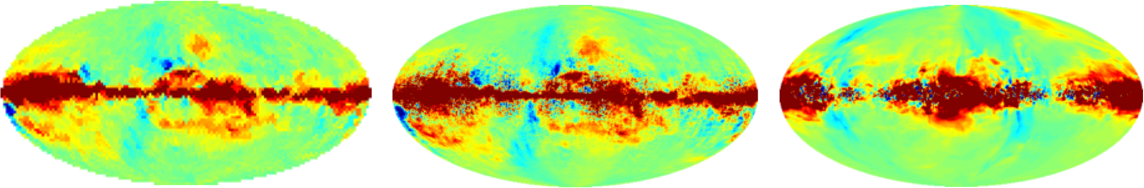
\includegraphics[width=.95\textwidth]{images/foregrounds_maps_planck_models}
%\vspace{-0.1in}
%\caption{\captiontext
%Foreground maps: \planck~measured sky (left) at 143~GHz, models at 155~GHz from PySM (middle)~\citep{thorne2018_pysm} and Galactic MHD simulations (right). \comor{The model generated by MHD simulations is only constrained to match \planck\ Galactic foregrounds spatial power spectra, not the actual spatial realization.} 
%\label{fig:pysm_foregrounds} }
%\end{center} 
%\vspace{-0.2in}
%\end{figure}

% To capture the potential impact of ...

%\comor{what exactly do you want to say here}
To test the results we constructed a variety of full-sky models~\citep{gnilc_memo}. All the models were broadly consistent with available data and with uncertainties from \wmap\ and \planck , but they differed in their degrees of Galactic emission complexity. Models included spectral parameters varying spatially and along the line of sight, anomalous microwave emission up to 2\% polarized, dust polarization that rotates slightly as a function of frequency because of projection effects, or dust \ac{SED}s that depart from a simple modified blackbody. All the foreground maps were generated at native resolution of 7\arcmin\ pixels~\citep{gorski/etal:2005}, with widely-used and thoroughly-tested map-generation codes~\citep{thorne2018_pysm,delabrouille/etal:2013}. 
%Fig.~\ref{fig:pysm_foregrounds} shows two of the eight models and data from \planck . \comor{The right panel is constructed to mimic the \planck\ Galactic emissions statistically. The middle panel is constructed to mimic the observed spatial distribution of Galactic emission. The differences between these and the \planck\ map illustrate that different realizations of the sky are allowed by current data, and highlight the level of current Galactic emission uncertainties. }

For each of the models, we added CMB signals in both intensity and polarization, matching a $\Lambda$CDM universe. The input inflationary signal was $r=0$, i.e., no signal, and the $BB$-lensing matched the level after 85\% delensing as forecast for PICO. Each of these sky models had 50 realizations of the PICO noise level. 
%, and 50 others had a level of $r=0.003$. \comor{do you want to talk about r=0.003?}
%\vspace{0.1in}
%\noindent{\bf Foreground Separation} \hspace{0.1in} 
The sky models were analyzed with a variety of foreground separation techniques.
%, which were based on the two broad categories described above. 
Because of limited resources for this study not all models were analyzed with all techniques, and not all realizations were used. 

%%%%%%%%%%%%%%%%%%%%%%%%%%%%%%%%%%%
\subsubsection{Results and Discussion}
\label{sec:foregrounds_results}
%%%%%%%%%%%%%%%%%%%%%%%%%%%%%%%%%%%

When using the PICO baseline noise levels with the analytic forecasts we find that $\sigma(r) = 2\times 10^{-5}$, a level that is five times lower than required ($\sigma(r) =1 \times 10^{-4}$, see SO1). We consider this forecast optimistic because it assumes strictly white noise, a specific model for the underlying foregrounds that has only eight parameters\footnote{Six amplitudes for the $Q$ and $U$ Stokes parameters of the CMB, dust, and synchrotron emission, and two spectral indices, for dust and synchrotron.} per $15 \times 15$~deg$^{2}$ pixel, and Gaussian parameter likelihood functions. The foregrounds may be more complex, requiring more  parameters (for example, spatially varying temperature for the dust, or more than a single spectral index per source of emission), and may have stronger spatial variations. Additionally, the parameter likelihoods may not be Gaussian. 
\begin{figure}[h]
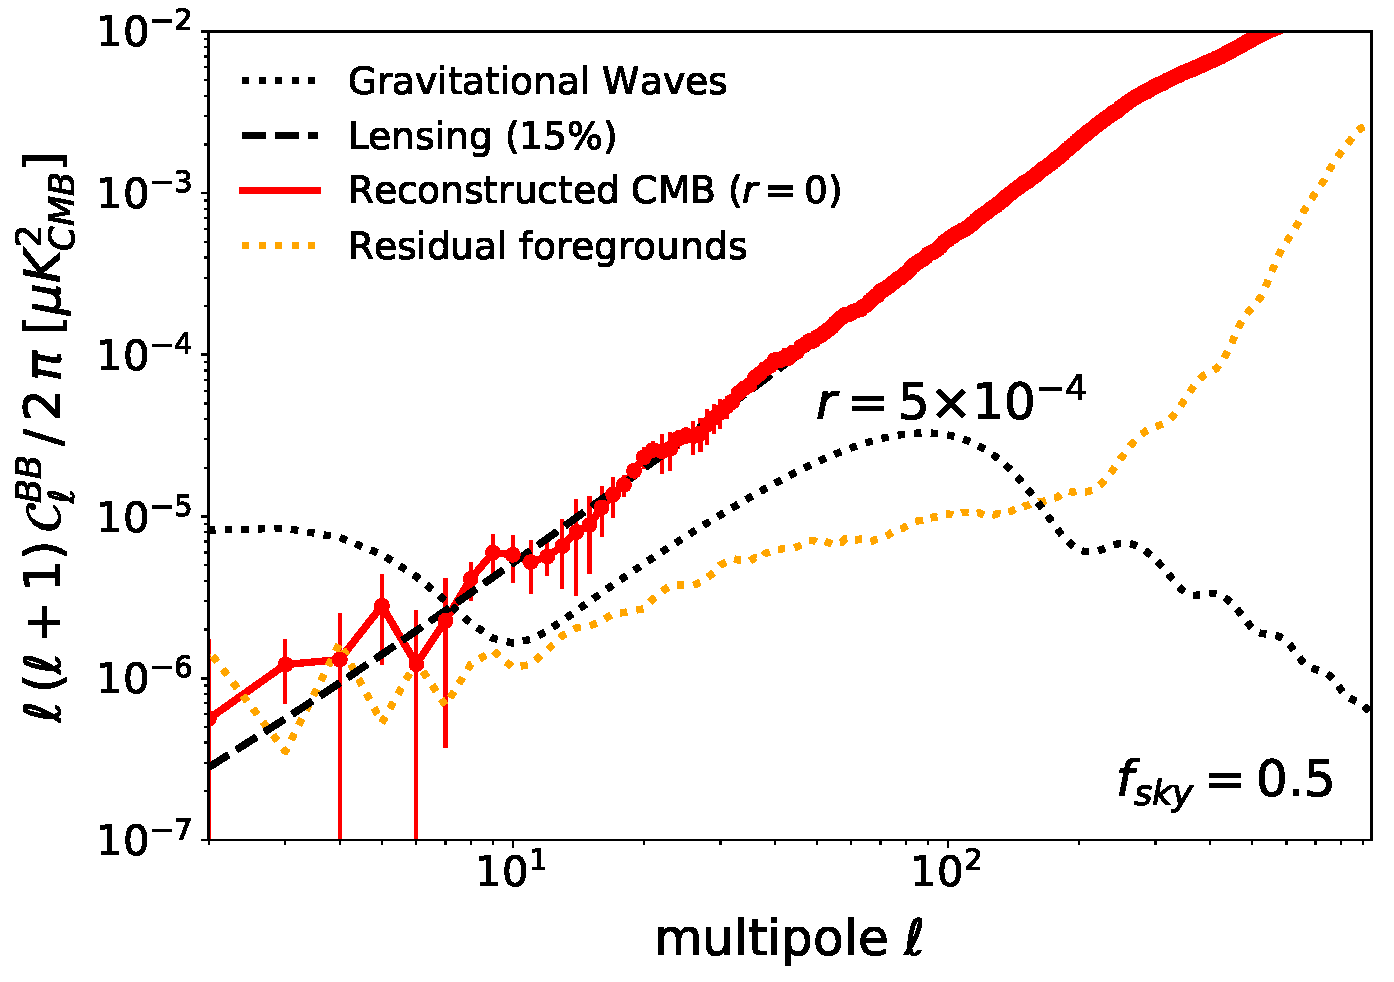
\includegraphics[width=3.2in]{images/gnilc_9092_residual.pdf}
\hspace{0.1in}
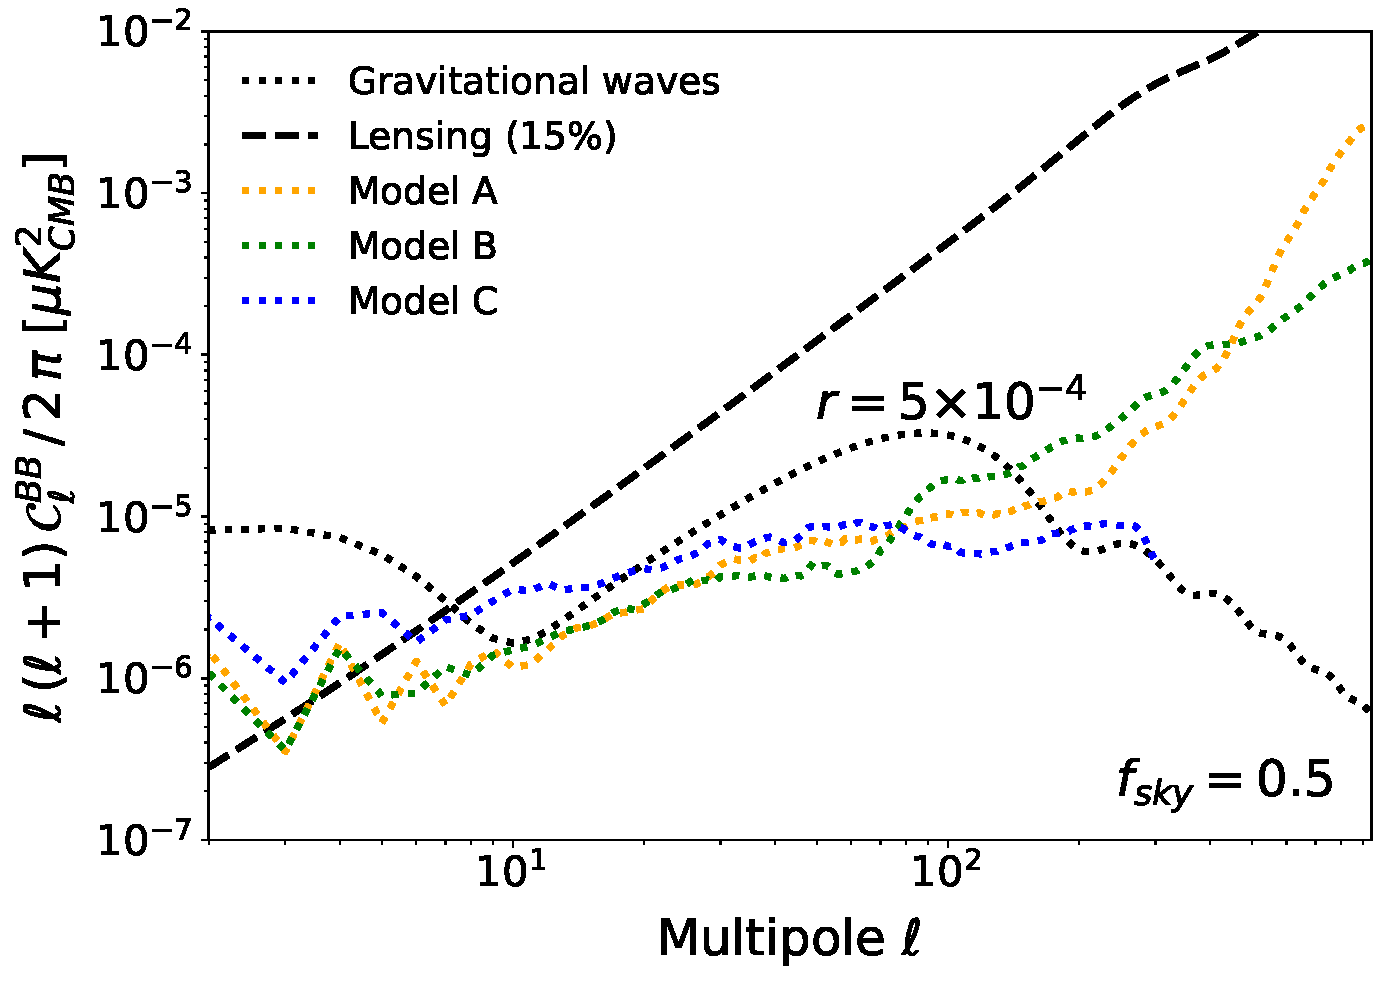
\includegraphics[width=3.2in]{images/gnilc_several_residuals.pdf}
\vspace{-0.3in}
\caption{\captiontext Angular power spectra of $BB$ due to the CMB and of residual foregrounds after an end-to-end map-based foreground-separation exercise. The PICO low noise levels and breadth in frequency coverage enable separation of model A foregrounds such that the residual foreground spectrum (left, yellow dotted) is a factor of ten (four) below a $BB$ inflationary signal with $r=5\times10^{-4}$ (black dotted) at $\ell=5 (80)$. Within errors, the recovered CMB (red) matches the input CMB, which consists of only lensing $BB$ (dashed black), over all angular scales $\ell \gtrsim 6$.  The results for model B are similar (right, green dots), while model C has somewhat higher residuals at low $\ell$. In this exercise we used 50\% of the sky. Lower foreground residual levels are obtainable with smaller, cleaner patches of $\sim$5\% of sky, which would reduce the residual foregrounds at $\ell \simeq 80$. 
\label{fig:nilc} } 
\vspace{-0.05in}
\end{figure}

%\begin{figure}[h]
%\hspace{0.in}
%\parbox{3.0in}{\centerline {
%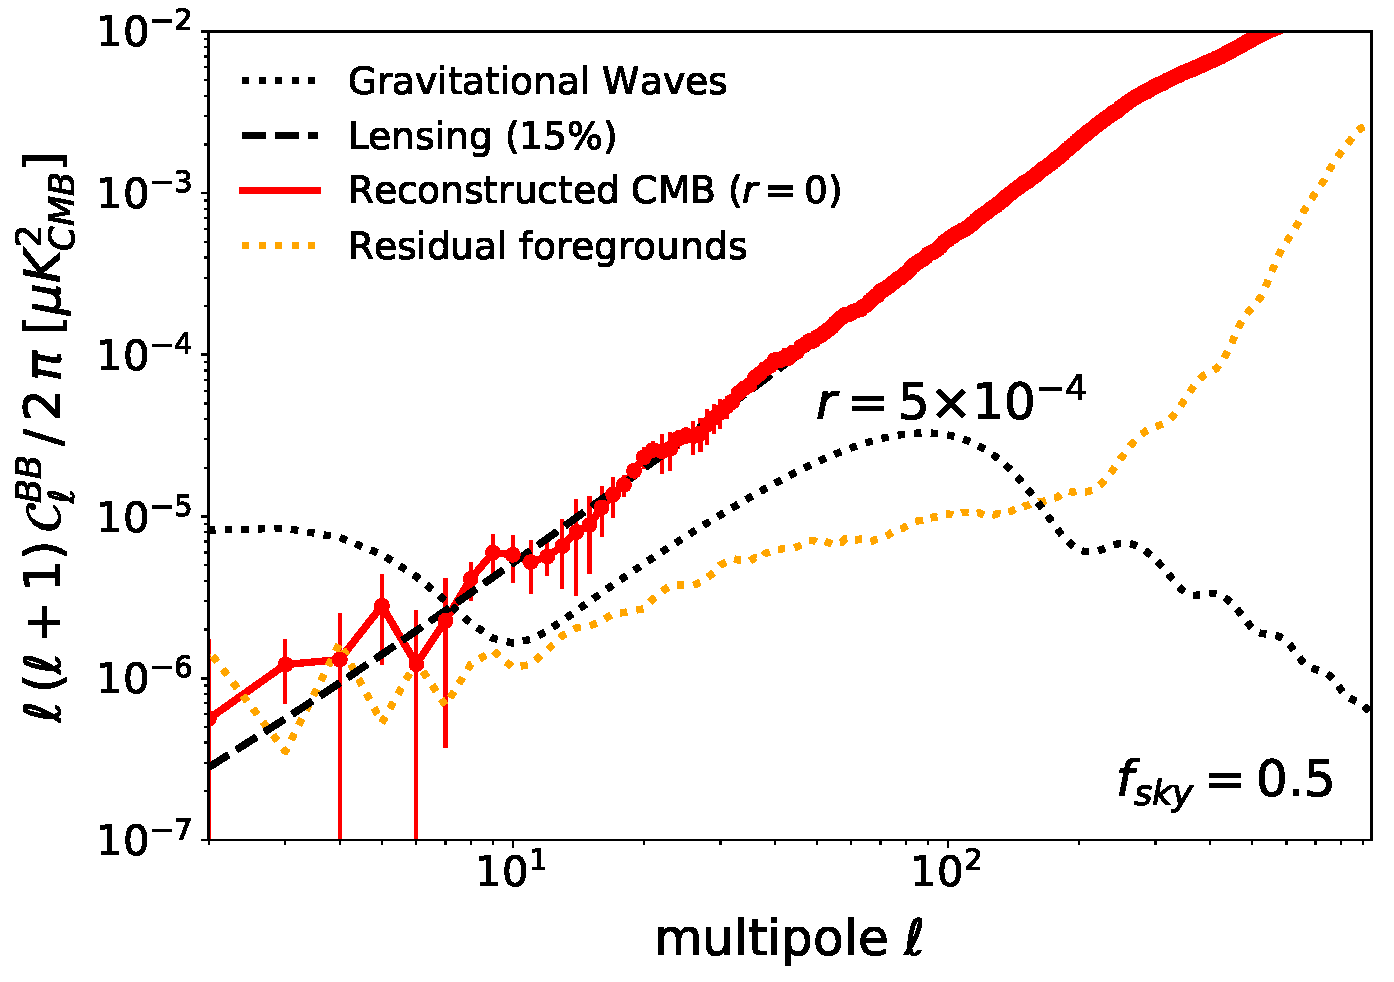
\includegraphics[width=3.3in]{images/gnilc_9092_residual.pdf}}}
%\hspace{0.2in}
%\parbox{3.2in}{
%\caption{\captiontext Angular power spectra of $BB$ due to the CMB and of residual foregrounds after an end-to-end map-based foreground-separation exercise. The PICO low noise levels and breadth in frequency coverage enable suppression of foregrounds such that the residual foreground  spectrum  (yellow dotted) is a factor of ten (four) \comblue{[which?]} below a $BB$ inflationary signal with $r=5\times10^{-4}$ (black dotted). Within errors, the recovered CMB (red) matches the input CMB, which consists of only lensing $BB$ (dashed black), over all angular scales $\ell \gtrsim 6$. In this exercise we used 50\% of the sky.  Lower foreground residual levels are obtainable with smaller, cleaner patches of $\sim$10\% of sky, which would reduce the residual foregrounds at $\ell \simeq 80$. 
%\label{fig:nilc} } }
%\vspace{-0.1in}
%\end{figure}

The `gold-standard' map-based simulations give initial evidence that the combination of PICO's sensitivity and broad frequency coverage are effective in foreground removal and that PICO will reach the requirement of $r = 5\times 10^{-4} \,(5\sigma)$. Figure~\ref{fig:nilc} shows the results of a foreground-separation exercise over 50\% of the sky, with three representative models of Galactic emissions, labeled A, B, and C~\citep{gnilc_memo}.  This exercise used GNILC, a non-parametric technique\cref{nonparametric}~\citep{gnilc}, tuned to give low foregrounds on the largest angular scales, that is, the lowest $\ell$ modes. The input CMB $BB$ signal, consisting of only lensing $B$-modes, is reconstructed within errors for all $\ell \gtrsim 5$.  With models A and B, the residual foreground $BB$ power spectrum, encoding the levels of remaining foreground emission after foreground separation is a factor of ten below an inflationary $BB$ signal for  $r = 5\times 10^{-4}$ at $\ell \simeq 4$.  These are the angular scales at which the inflationary signal is stronger than the signal from lensing.  Comparing models' A and B residual foregrounds at this $\ell$ range to the input $BB$ foregrounds at, for example, 155~GHz (Fig.~\ref{fig:clbb}) we find a strong suppression (a factor of 1000 in temperature), which is a consequence of PICO's multiplicity of bands and high sensitivity.  The residual in model C is a factor of 2 higher than for A and B at $\ell <30$. Of all models, this model is least constrained to match existing sky measurements~\citep{gnilc_memo}.  


% is a factor of 50 below the CMB at $\ell=100$ and a factor of five at $\ell=10$. 

%The `gold-standard' map-based simulations give initial evidence that the combination of PICO's sensitivity and broad frequency coverage are effective in foreground removal and that PICO will reach the requirement of $r = 5\times 10^{-4} (5\sigma)$. Fig.~\ref{fig:nilc} shows the results of a foreground-separation exercise over 50\% of the sky, with three representative models of Galactic emissions, labeled A, B, and C~\citep{gnilc_memo}.  This exercise used GNILC, one of the non-parametric techniques\cref{nonparametric}~\citep{gnilc}, tuned to give low foregrounds on the largest angular scales, that is, the lowest $\ell$ modes. The input CMB $BB$ signal, consisting of only lensing $B$-modes, is reconstructed within errors for all $\ell \gtrsim 6$~\citep{gnilc_memo}.  With models A and B the residual foreground $BB$ power spectrum, encoding the levels of remaining foreground emission after foreground separation, is a factor of 50 below the CMB at $\ell=100$ and a factor of five at $\ell=10$. Most importantly, the residual foreground is a factor of ten below an inflationary $BB$ signal for  $r = 5\times 10^{-4}$ at $\ell \simeq 4$.  These are the angular scales at which the inflationary signal is stronger than the signal from lensing.  Comparing models' A and B residual foregrounds at this $\ell =4 $ to the input $BB$ foregrounds at, for example, 155~GHz (Fig.~\ref{fig:clbb}) we find a suppression of $\sim10^{6}$ in $\mu$K$^{2}$ (a factor of 1000 in temperature), which is a consequence of using {\it all} of PICO bands.  The residual in model C is a factor of 2 higher than for A and B at $\ell <30$. Of all models, this model is least constrained to match existing sky measurements~\citep{gnilc_memo}.  

At intermediate angular scales, $\ell \simeq 80$, the residual foreground is a factor of four lower than the inflationary signal. We expect lower residuals when the GNILC analysis is optimized for this $\ell$ range. Furthermore, for reconstructing signals at this $\ell$ range, it is sufficient to analyze data from smaller $\sim$5\% regions of the sky. These will have lower mean foreground levels, making the foreground-separation exercise easier, and pushing residuals to levels lower than demonstrated for 50\% of the sky. With its full-sky coverage, PICO will have access to several independent 5\% sky patches, and will thus make several independent measurements of its $r$ target. 

%Map-based simulations that were carried out for the forthcoming CMB-S4 experiment have shown that with a much narrower frequency band coverage, extending only between \comor{20?} and 300~GHz, the experiment can reach a level of $\sigma(r) = 0.0005$ in a 3\%-size clean patch of the sky. Using 

%\comor{connect to Jonathan's analysis?} 

%There is other evidence that PICO could reach its stated target of $\sigma(r) = 0.0001$. Map-based simulations that were carried out for the forthcoming CMB-S4 experiment have shown that it can reach levels of $\sigma(r) = 0.0005$ in small, 3\%-size, clean patches of the sky. 
%The analysis only used frequencies up to 300~GHz. 
%The PICO noise level per sky pixel is similar to that of CMB-S4, but PICO will have {\it full} sky coverage and thus access to {\it all} the clean patches available. Data from \planck\ indicate that there are approximately ten %\comor{check!} 
%patches as clean, or cleaner than those used for the CMB-S4 analysis, indicating that PICO's $\sigma(r)$ could be about three times more stringent. This scaling is very conservative because it only assumes CMB-S4's much narrower breadth of frequency coverage and its seven bands; % \comor{check}; 
%it neglects PICOs much stronger rejection of foregrounds with 21 bands and up to 800~GHz.  We note that if there {\it is} a detection of the \ac{IGW} signal with $r=0.001$, PICO will make it with high significance in multiple independent patches of the sky. 


%It is an advantage for PICO  which correspond to   The residual is  is  using realistic input foregrounds and an input polarized CMB that has bothonly $B$-mode due to lensingafter separation of foregrounds sky model with an input a result one of the sky models and with an input \ac{IGW} of $r=0.003$. Residual foregrounds are below the cosmological signal over the important low $\ell$ range, where foregrounds are strongest. The residual spectra would likely be lower when analysis is carried out on only 50 or 40\% of the sky, rather than the 60\% used here. 

Some of our results validate the need for a broad frequency coverage with a strong lever arm on Galactic emissions outside the primary CMB bands. Figure~\ref{fig:commander} shows that removing several of PICO's frequency bands, particularly those that monitor dust at high frequencies and synchrotron at low frequencies, can significantly bias the extracted $BB$ power spectrum, especially at the lowest multipoles. In this exercise the input CMB contained the lensing signal {\it and} an inflationary signal with $r=0.001$, and a parametric technique was used for foreground separation~\citep{eriksen/etal:2008,gnilc_memo}. 

%While our results are encouraging, as they suggest that PICO's frequency coverage and sensitivity will be adequate for this level  of $r$, more work should be invested to gain complete confidence. 
While these results suggest that PICO's frequency coverage and sensitivity will be adequate for this level of $r$,  more work should be invested to gain complete confidence. For example, some of the other sky models yield a level of residual foregrounds that would result in biased measurements, reflecting larger values of $r$; and some of the foreground-separation techniques appear to give consistently higher foreground residuals than others. To make progress, it is important to continue the simulations and algorithm development program, by: running numerous realizations of different sky models and analyzing them with various approaches; optimizing sky masks; and potentially using a combination of techniques to handle large, intermediate, and small angular scale foregrounds differently. It would also be valuable to continue measurements of Galactic emissions with ground- and balloon-based experiments to further reduce the current level of Galactic emission uncertainties.  
\begin{figure}
%\hspace{-0.1in}
%\parbox{4.5in}
\centering
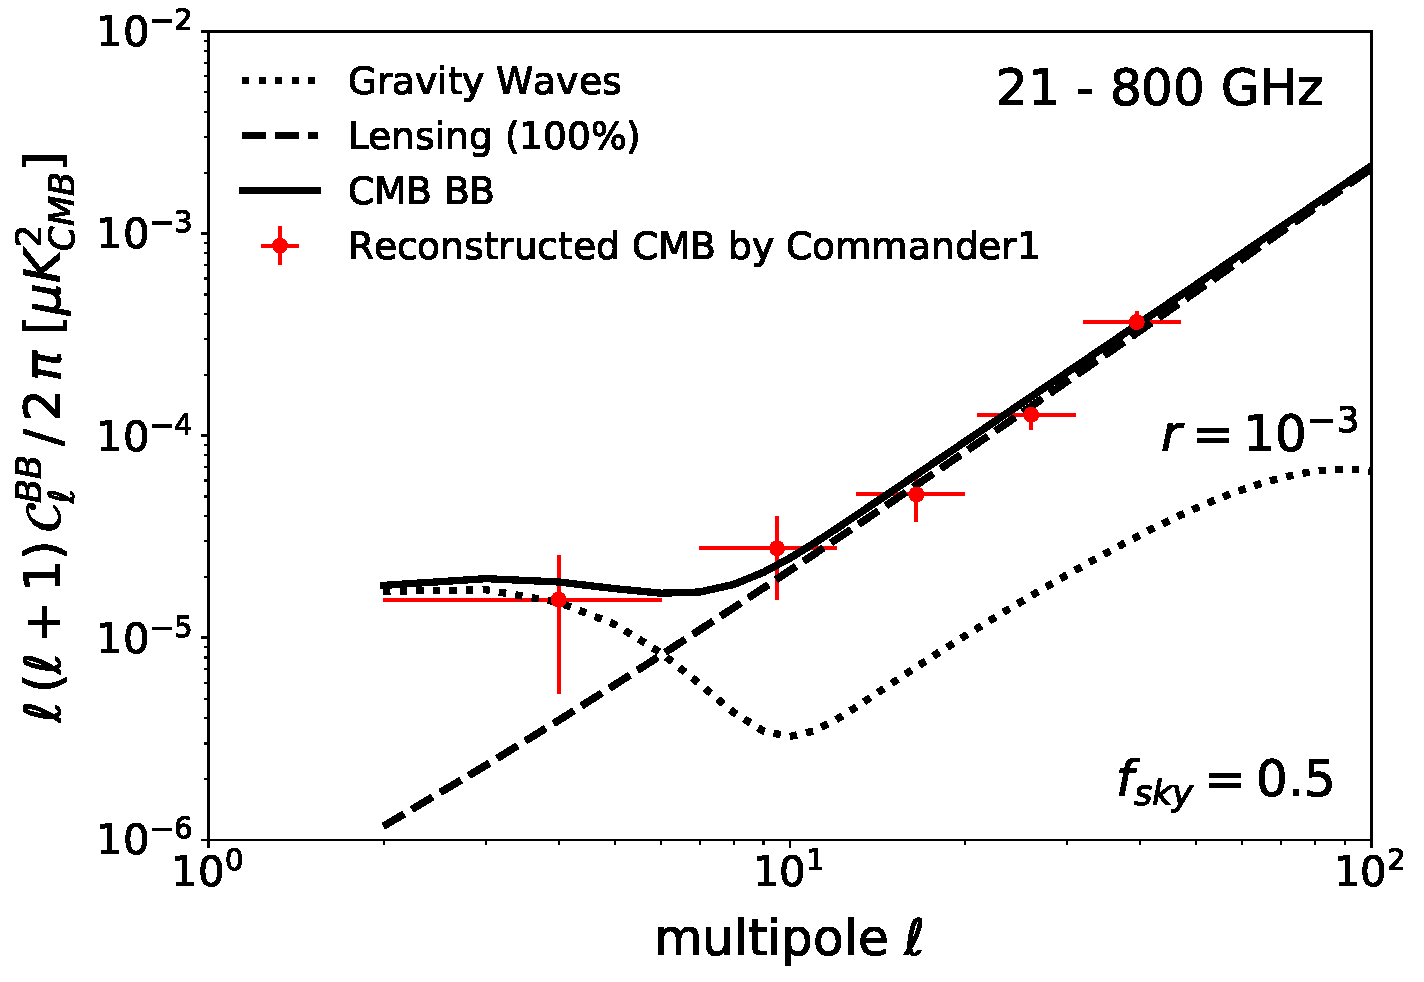
\includegraphics[width=3in]{images/commander_pico_baseline.pdf}
\hspace{-0.0in}
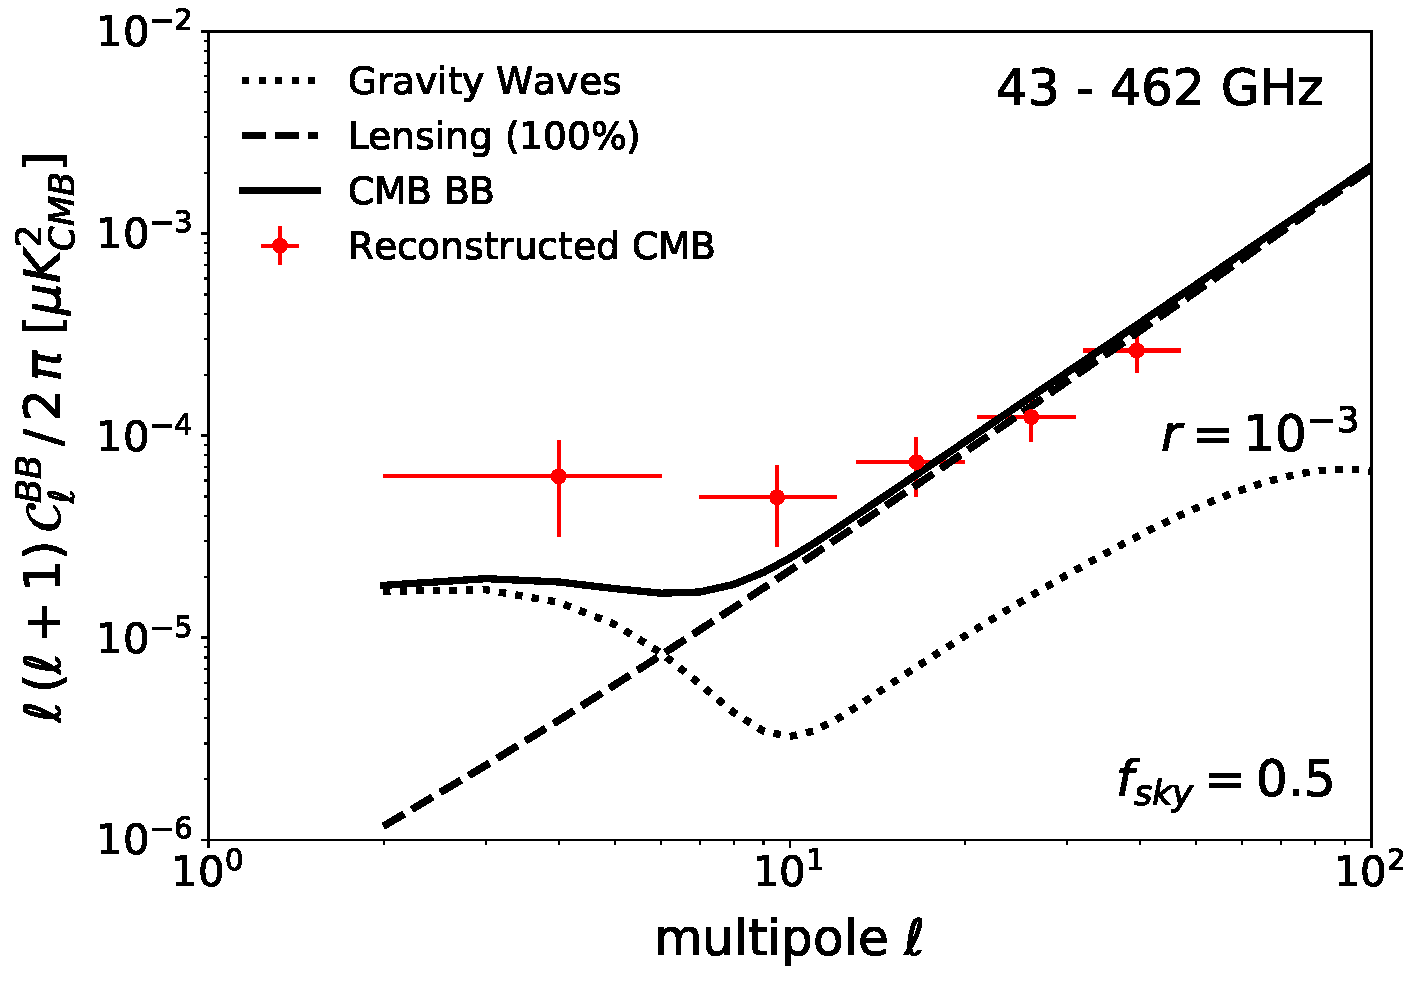
\includegraphics[width=3in]{images/commander_pico_descoped.pdf}
%\hspace{0.in}
%\parbox{2.0in}{
\vspace{-0.1in}
\caption{\captiontext
{\bf Left:} Foreground separation with all of PICO's 21 frequency bands recovers the input CMB $BB$ power spectrum (solid black) without bias (red). The input CMB spectrum has a contribution from lensing (dashed) and an inflationary signal with $r=0.001$ (dotted). This exercise uses a parametric approach~\citep{eriksen/etal:2008} with foregrounds varying on 4$^\circ$ pixels, and using 50\% sky fraction. {\bf Right:} Running the same foreground separation algorithm on the same sky but using only PICO's bands between 43 and 462~GHz produces an output spectrum (red) that is biased at low multipoles relative to the input. With real data, such a bias would be erroneously interpreted as a higher value of $r$. 
\label{fig:commander}}
\vspace{-0.1in}
\end{figure}


\end{document}

%\begin{figure}[!htb]
%\centering
%
\includegraphics[width=4cm]{images/example}
%\caption{example}
%\label{fig:im_3}
%\end{figure}

%The most important lesson arising from our exercise is that more work is required to ascertain that levels of $r \lesssim 0.001$ can be determined robustly on the largest angular scales, that is from the reionization peak.  Fig.~\ref{fig:nilc} shows results from the NILC analysis. For several of the sky models the power spectra of the residual level of foregrounds -- that is the level of foregrounds remaining in the map after foreground separation -- is below the cosmological \ac{IGW} level with $r =0.003$. For a minority of the models, the residual is higher at $\ell \lesssim 20$. Results from GNILC, shown in Fig.~\ref{fig:gnilc}, are similar. In all cases, the analyses are carried out using 60\% of the sky, the results shown are from one realization, and that no further optimization of the basic foreground separation technique has yet been applied. 

%More work is also required to understand the necessary span of frequencies required. Fig.~\ref{fig:psm_mr} shows that removing several of PICO's frequency bands, in this case the three highest, significantly biases the extracted $BB$ power spectrum, particularly at the lowest $\ell$ values. This result should not be interpreted as conclusively demonstrating that a frequency span up to 800 GHz has been proven to be essential. At this point of time, different input sky models, coupled to different foreground separation techniques may yield different results. Rather, the conclusion is that further improvement in our modeling and analysis is required. 



%The baseline design of PICO has 21 channels observing the sky in the 20\,GHz to 800\,GHz frequency range (Fig.~\ref{fig:pico-channels-and-fg}). By analysing how the total emission varies across frequency bands, one can infer the detailed emission properties of the various emission components, form linear combinations of the observations that maximise the contribution of a component of interest while minimising contamination by the others and by instrumental noise, and understand the properties of the foregrounds to evaluate potential residuals in the CMB B-mode map. Various such techniques have been successfully used in previous CMB observations such as those of the Planck mission. Building on this existing expertise, we have carried out map based simulations within a ``data challenge'' framework to assess the capacity of PICO to measure the main signal of interest (CMB primordial B-modes). In this process one group prepares sets of simulated maps for different models of foreground emission of varying complexity from optimistic to pessimistic, which are placed in a shared area. These are then re-analyzed by multiple individuals and groups employing various different component separation algorithms.

